\section{EELS analyses and TMD nanostructures}
\label{sec:tmdeels}

In this work, we will apply our machine learning method to the study
of the low-loss EELS region of a specific type of WS$_2$ nanostructures presented in~\cite{SabryaWS2},
characterised by a flower-like morphology and a 2H/3R mixed polytypism.
%
WS$_2$ is a member of the transition metal dichalcogenide (TMD) family, which in turn
belongs to a class of materials known as two-dimensional, van der Waals, or simply layered materials.
%
These materials are
characterised by the remarkable property of being fully functional down to a single atomic layer.
%
In order to render the present work self-contained and accessible to a wider audience,
here we review the basic concepts underlying  the EELS technique, and then
present the main features of the WS$_2$ nanoflowers that will be studied in the subsequent sections.

\subsection{EELS and its ZLP in a nutshell}
\label{sec:eels}

Electron energy loss spectroscopy is a TEM-based method
whereby an electron-transparent sample is illuminated by a 
beam of energetic electrons.
%
Subsequent to the crossing of
the specimen, the scattered electron beam is focused by a magnetic prism
towards a spectrometer where the distribution of electron energy losses $\Delta E$ can be recorded.
%
The schematic illustration of a typical EELS setup is shown in the left panel of Fig.~\ref{fig:EELS}.
%
EEL spectra can be recorded either in the Scanning Transmission Electron Microscopy (STEM) mode
or in the conventional TEM (c-TEM) setup.
%
Thanks to recent progress in TEM instrumentation and data acquisition, state-of-the-art EELS analyses benefit from
a highly competitive energy (spectral) resolution combined with an unparalleled spatial resolution.

%%%%%%%%%%%%%%%%%%%%%%%%%%%%%%%%%%%%%%%%%%%%%%%
\begin{figure}[t]
  \centering
  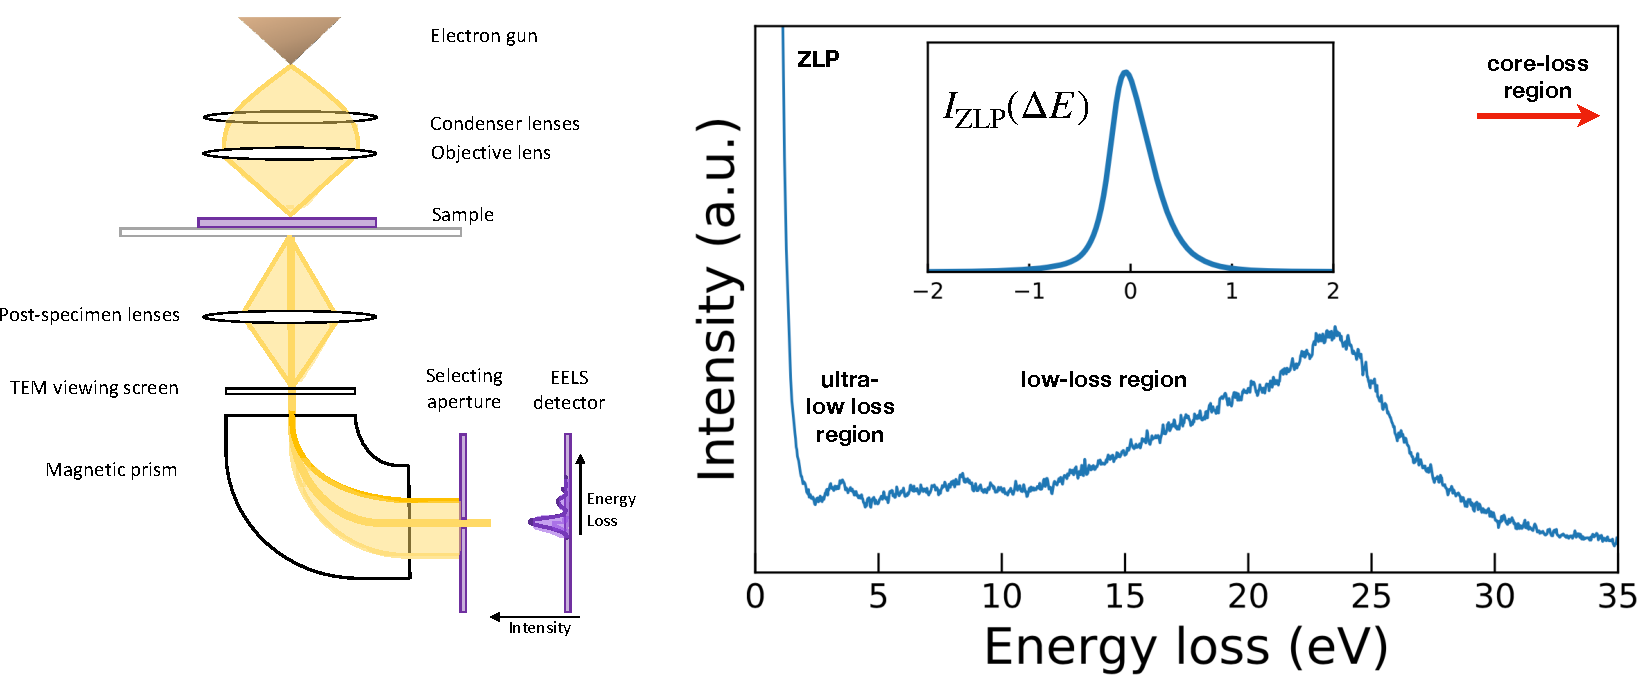
\includegraphics[width=0.40\textwidth,angle=-90]{plots/EELS.pdf}
  \caption{Left: schematic representation of the STEM-EELS setup.
    %
    A magnetic
    prism is used to deflect the electron beam after it has crossed the sample,
   allowing the distribution of energy losses $\Delta E$ to be recorded
    with a spectrometer.
    %
    Right: a representative low-loss EEL spectrum acquired 
    on a WS$_2$ nanoflower~\cite{SabryaWS2} with
    the inset displaying the corresponding ZLP.
  }
  \label{fig:EELS}
\end{figure}
%%%%%%%%%%%%%%%%%%%%%%%%%%%%%%%%%%%%%%%%%%%%%%%%5

EELS spectra can be approximately divided into three main regions.
%
The first is the zero-loss region, centered around $\Delta E=0$
and containing the contributions from both elastic scatterings
as well as those from electrons that have not interacted with the
sample.
%
This region is characterised by the strong and narrow ZLP
which dominates over the contribution
from inelastic scatterings.
%
The second region is the low-loss region, defined for energy losses
$\Delta E \lsim 50$ eV, which contains information
about several important features such as plasmons, excitons, phonons, and
intra-band transitions.
%
Of particular relevance in this context is the ultra-low loss region, characterised by $\Delta E \simeq$ few eV.
%
There, the contributions of the ZLP and those from inelastic interactions
become comparable.
%
The regime for which $\Delta E \gsim 50$ eV is then known as the core-loss region and
provides compositional information
on the materials that constitute the specimen.

The right panel of Fig.~\ref{fig:EELS} displays
a representative EELS spectrum in the region $\Delta E \le 35$ eV, recorded
in one of the WS$_2$ nanoflowers of~\cite{SabryaWS2}.
%
The inset displays the ZLP, illustrating how nearby $\Delta E\simeq 0$
its size is larger than the contribution from the inelastic scatterings
off the sample by several orders of magnitude.
%
Carefully disentangling these two contributions 
is essential for the physical interpretation of EEL spectra in the ultra-low-loss region.

The magnitude and shape of the ZLP intensity is known to depend not only on the specific values
of the electron energy loss $\Delta E$, but also on other operation parameters
of the TEM such as the electron beam energy $E_{b}$, the exposure time
$t_{\rm exp}$, the aperture width, and the use of a monochromator.
%
Since it is not possible to compute the dependence of the ZLP on $\Delta E$
and the other operation parameters from first principles,
reliance on specific models seems to be unavoidable.
%
This implies that one cannot measure the ZLP for a given operating
condition, for instance a high beam voltage of 200 kV, and expect to reproduce
the ZLP intensity distribution
associated to different conditions, such as a lower beam voltage of 60 kV,
without introducing model assumptions.

Several attempts to describe the ZLP distribution have reported
some success at predicting the main intensity of the peak, 
but in the tails discrepancies are as large as several tens of percent~\cite{Bangert:2003}.
%
The standard method for background subtraction
is to fit a power law to the tails, however this approach is not suitable in
many circumstances~\cite{Hachtel:2018, Tenailleau:1992, Reed:2002, Bosman:2006}.
%
Further, even for nominally identical operating conditions, the intensity of the ZLP
will in general vary due to {\it e.g.} external perturbations such as electric or magnetic fields~\cite{Rafferty:2000},
the stability of the microscope and spectrometer electronics~\cite{Kothleitner:2003}, the local
environment (possibly exposed to mechanical, pressure and temperature fluctuations) 
and spectral aberrations~\cite{Egerton:1996}. 
%
Any robust statistical model for the ZLP should thus account for this irreducible source of uncertainties.

\subsection{TMD materials and WS$_2$ nanoflowers}
\label{sec:tmd}

In this work we will apply our ZLP parametrisation strategy
 to a novel class of recently presented WS$_2$ nanostructures known
as nanoflowers~\cite{SabryaWS2}.
%
WS$_2$ belongs to the TMD class of layered materials together with {\it e.g.}
MoS$_2$ and WSe$_2$.
%
TMD materials are of the form MX$_2$, where M is a 
transition metal atom (such as Mo or W) and X a chalcogen atom (such as S, Se, or Te). 
%
The characteristic crystalline structure of TMDs is such that
one layer of M atoms is sandwiched between two layers of X atoms.

The local electronic structure of TMDs strongly depends on the coordination 
between the transition metal atoms, giving rise to an array of remarkable electronic
and magnetic properties~\cite{Chhowalla:2013}.
%
Furthermore, the properties of this class of materials vary significantly
with their thickness, for instance MoS$_2$ exhibits an indirect bandgap
in the bulk form which becomes direct at the monolayer level~\cite{Splendiani:2010}.
%
The tunability of their electronic properties and the associated
potential applications in nano-electronics make TMD materials highly attractive for fundamental research. 

As for other TMD materials, WS$_2$ adopts a layered structure 
by stacking atomic layers of S-W-S in a sandwich-like configuration. 
%
Although the interaction between adjacent layers is a weak Van der Waals 
force, the dependence of the interlayer interactions on the stacking 
order of WS$_2$ can be significant.
%
Therefore, modulating the stacking arrangement of WS$_2$ layers (as well
as their relative orientation)
represents a promising handle to tailor the resulting local electronic properties.
%
WS$_2$ also exhibits a marked thickness dependence of
its properties, with an indirect-to-direct bandgap transition when going
from bulk to bilayer or monolayer form.
%
The effects of this transition are manifested for example as enhanced
photoluminescence in monolayer WS$_2$, whereas greatly suppressed emission is observed in
the corresponding bulk form~\cite{Zhao2013}.
%
Further applications of this material include storage of hydrogen 
and lithium for batteries~\cite{Bhandavat:2012}.

%%%%%%%%%%%%%%%%%%%%%%%%%%%%%%%%%%%%%%%%%%%%%%%%%%%%%%%%%%%%%%%%%%%%%%%%%%%%%%%
\begin{figure}[t]
    \centering
    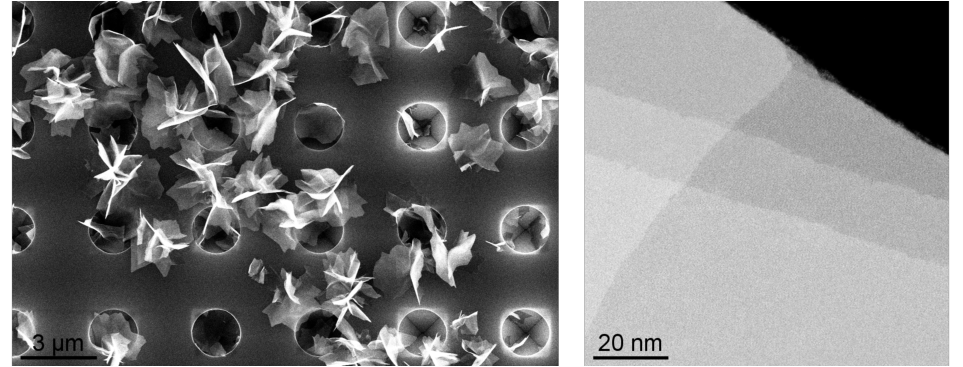
\includegraphics[width=0.99\textwidth]{plots/TEMwE-full-figure-withscales-centred-1.pdf}
    \caption{Left: low-magnification TEM image of the WS$_2$ nanoflowers
      grown on top of a holey Si/SiN substrate.
      %
      Right: the magnification of a
      representative petal
      of a nanoflower, where the black region corresponds to the vacuum (no substrate)
      and the difference in contrast indicates terraces of varying thickness.
       }
    \label{fig:nanoflowers}
\end{figure}
%%%%%%%%%%%%%%%%%%%%%%%%%%%%%%%%%%%%%%%%%%%%%%%%%%%%%%%%%%%%%%%%%%%%%%%%%%%%%%%%%%5

A low-magnification TEM image of the WS$_2$ nanoflowers is displayed
in the left panel of Fig.~\ref{fig:nanoflowers}.
%
These nanostructures are grown directly on top of a holey TEM substrate.
%
The right panel shows the magnification of a
representative petal
of a nanoflower, where
the difference in contrast indicates terraces of varying thickness.
%
Note that the black region corresponds to the vacuum, that is, without
substrate underneath.
%
These WS$_2$ nanoflowers exhibit a wide variety of thicknesses, orientations
and crystalline structures, therefore representing an ideal laboratory to correlate
structural morphology in WS$_2$ with electronic properties at the nanoscale.
%
Importantly, these nanoflowers are characterised by a mixed crystalline structure,
in particular 2H/3R polytypism.
%
This implies that different stacking types tend to coexist,  affecting
the interlayer interactions within WS$_2$
and thus modifying the resulting physical properties~\cite{Na:2018}.
%
One specific consequence of such variations in the stacking patterns is the appearance of
spontaneous electrical polarization, leading to modifications of the 
electronic band structure and thus of the bandgap~\cite{Lee:2016,XIA20171}.



As mentioned above, one of the most interesting properties of  WS$_2$ is
that when the material
is thinned down to a single monolayer its indirect bandgap of
$E_{\rm BG}\simeq 1.4$ eV
switches to a direct bandgap of approximately $E_{\rm BG}\simeq 2.1$ eV.
%
It has been found that the type and magnitude of the  WS$_2$  bandgap
depends quite sensitively on the crystalline structure and
the number of layers that constitute the material.
%
In Table~\ref{table:bgvalues} we collect
representative results for the determination of the bandgap energy $E_{\rm BG}$
and its type in WS$_2$, obtained by means of different experimental and theoretical techniques.
%
 For each reference we indicate separately the bulk results and those
obtained at the monolayer level.
%
We note that for the latter case there is a fair spread of results in the
value of $E_{\rm BG}$, reflecting the challenges of its accurate determination.

 
%%%%%%%%%%%%%%%%%%%%%%%%%%%%%%%%%%%%%%%%%%%%%%%%%%%%%%%%%%%%%%%%%%%%%%%%%%%%%%%%%%%%%
\begin{table}[t]
  \small
  \begin{centering}
   \renewcommand{\arraystretch}{1.20}
\begin{tabular}{ccccc}
\br
Reference                       & Thickness & $E_{\rm BG}$ (eV)  & bandgap type  & Technique \\
\mr
{\cite{Braga:2012}} & bulk   & $1.4\pm0.07$            & indirect  & {Gate-voltage dependence}  \\
\mr
\multirow{2}{*}{\cite{Jo:2014}}                 & monolayer  & $2.14 $         & direct  & \multirow{2}{*}{Gate-voltage dependence}        \\
& bulk & $1.40 $    & indirect              \\
\mr

\multirow{2}{*}{\cite{Gusakova:2007}} & monolayer   & $2.03\pm0.03$            & direct  & \multirow{2}{*}{Density Functional Theory}  \\
& bulk & $1.32\pm0.03 $            & indirect     \\
\mr
\multirow{2}{*}{\cite{Kam:1982}}                  & monolayer  & $1.76\pm0.03 $      & direct    & \multirow{2}{*}{Absorption edge coefficient fitting}         \\
& bulk & $1.35 $          & indirect        \\
\mr
\cite{Shi:2013}                &monolayer   & $2.21\pm0.3 $         & direct  & Bethe-Salpeter equation (BSE)        \\                 \br                                         
\end{tabular}
\vspace{0.27cm}
\caption{Representative results for the determination of the bandgap energy $E_{\rm BG}$
  and its type in WS$_2$, obtained by means of different experimental and theoretical techniques.
  %
  For each reference we indicate separately the bulk results and those
  obtained at the monolayer level.}
    \label{table:bgvalues}
    \end{centering}
\end{table}
%%%%%%%%%%%%%%%%%%%%%%%%%%%%%%%%%%%%%%%%%%%%%%%%%%%%%%%%%%%%%%%%%%%%%%%%%%%%%%%%%%%%%%
